\documentclass[a4paper,10pt]{article}
\usepackage[utf8]{inputenc}
\usepackage[T1]{fontenc}
\usepackage[french]{babel}
\usepackage{textcomp}
\usepackage{listings}
\usepackage{pdfpages}
\usepackage{array}
\usepackage{titling}
\usepackage{geometry}

\geometry{hmargin=2.5cm,vmargin=1.5cm}
\setlength{\hoffset}{-18pt}        
\setlength{\oddsidemargin}{0pt} % Marge gauche sur pages impaires
\setlength{\evensidemargin}{9pt} % Marge gauche sur pages paires
\setlength{\marginparwidth}{54pt} % Largeur de note dans la marge
\setlength{\textwidth}{481pt} % Largeur de la zone de texte (17cm)
\setlength{\marginparsep}{2pt} % Séparation de la marge
\setlength{\topmargin}{0pt} % Pas de marge en haut
\setlength{\headheight}{6pt} % Haut de page
\setlength{\headsep}{10pt} % Entre le haut de page et le texte
\setlength{\footskip}{27pt} % Bas de page + séparation
\setlength{\textheight}{708pt} % Hauteur de la zone de texte (25cm)

\setlength{\droptitle}{-4cm}
\title{Synthèse - Machine Learning}
\author{Léa Calem - Fatima Layla - Laureline Martin}

\begin{document}

\maketitle
	
\section{Description du jeu de données}
	\subsection{Les données}
	% \subsubsection{Modélisation des données sous forme de matrice}
		Nous disposons de 14 000 images représentant soit des t-shirts/tops, soit des robes. La classe $C_1 =$ \{0 T-shirt/top\} et la classe $C_2 =$ \{3 Dress\}.
		\begin{itemize}
			\item 7 000 images de la classe $C_1$
			\item 7 000 images de la classe $C_2$
		\end{itemize}
		Les images sont de taille 28x28 pixels (784 pixels) et sont composées de niveau de gris (valeur allant de 0 à 255). Sur ces images, seul l’objet est coloré donc le reste de l’image est en blanc, la valeur des pixels à 0.\\
		Nous avons remarqué que certains vêtements sur certaines images sont très difficilement reconnaissables. En effet, certains tops ressemblent à des robes (et inversement) et certaines images contiennent plusieurs vêtement superposés. Ces images sont très difficiles à évaluer et à classifier.\\
		Ces données sont issues des classes 0 et 3 du jeu données Fashion-MNIST (http://www.openml.org/d/40996). 
	\subsection{Séparation des jeux de données}
		\begin{enumerate}
			\item Données d’entraînement : sous-ensemble de données destiné à l’apprentissage du modèle. Nous utilisons 80\% des données pour l'apprentissage, soit 11 200 images.
			\item Données de test : sous-ensemble de données destiné à l’évaluation du modèle (ce jeu de données ne doit en aucun cas être utilisé lors de la conception du modèle). Nous utilisons 20\% des données, soit 2 800 images.
		\end{enumerate}
	\subsection{Description statistique}
		\begin{minipage}{0.55\linewidth}
			Ci-contre, un graphe représente un échantillon de 398 images (199 de la classe $C_1$ et 199 de $C_2$) avec comme axes les différents rapports décrits dans la section 2.2 Paramètres.
			\begin{itemize}
				\item Rouge : classe $C_1$
				\item Gris : classe $C_2$
			\end{itemize}
		\end{minipage}\hfill
		\begin{minipage}{0.4\linewidth}
			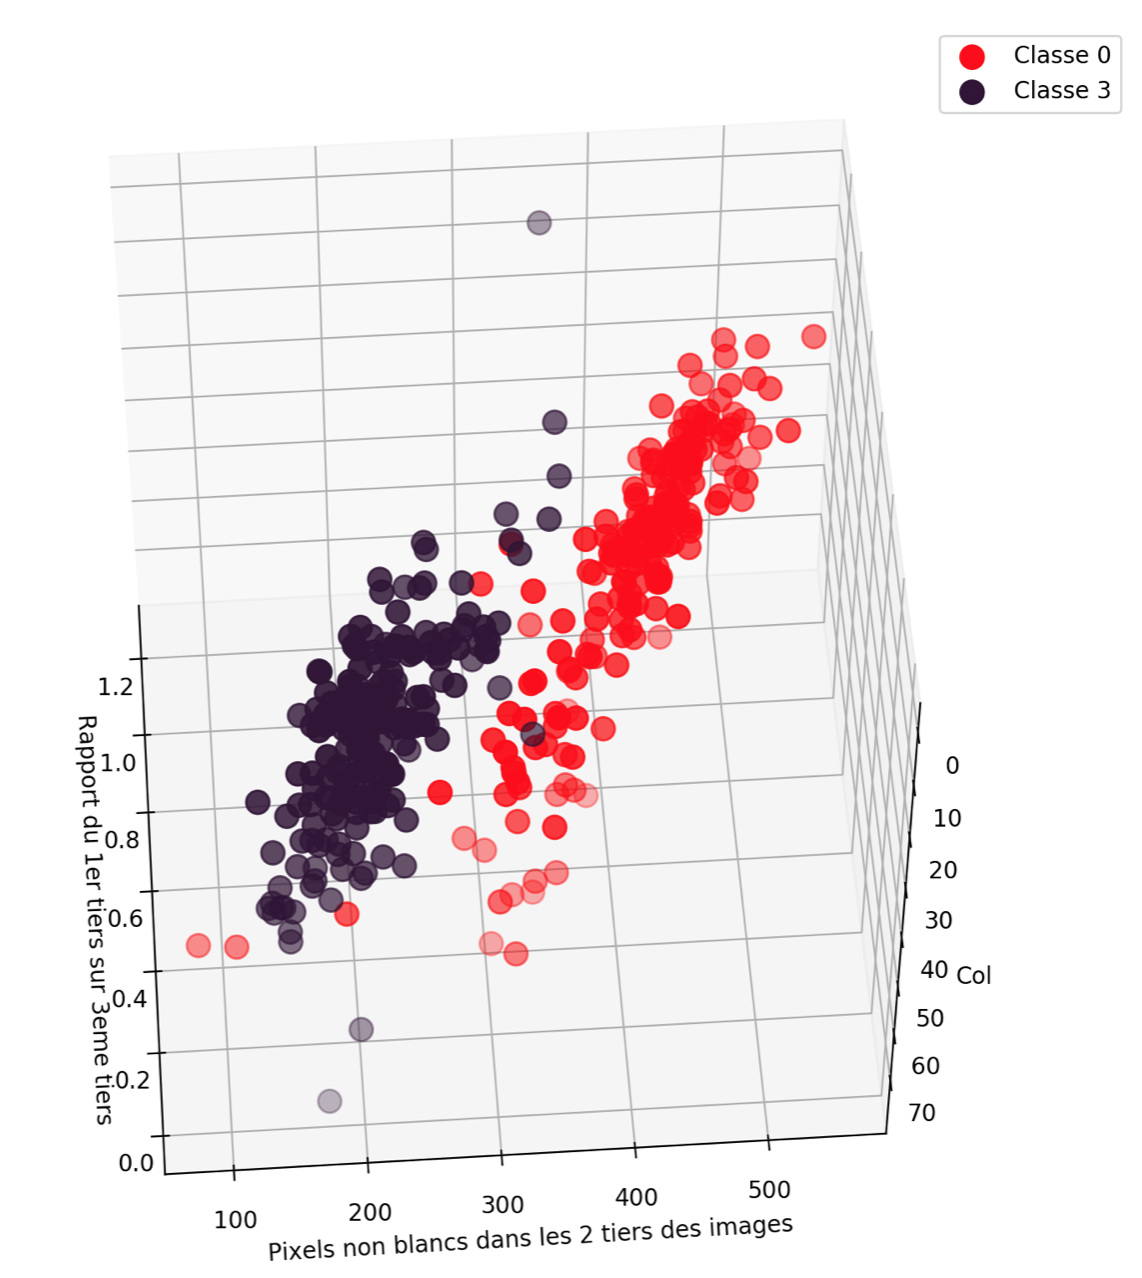
\includegraphics[scale = 0.2]{fichiers/rapport.PNG}
		\end{minipage}\hfill

\newpage
\section{Méthodologie}
	\subsection{Méthodologie générale}
		Dans ce projet, nous allons classifier des images en deux catégories : t-shirts/tops ou robes.\\
		Les méthodes d'apprentissages que nous allons utiliser sont de type supervisées car nos données sont déjà annotées :
		$$ S = {(x_i, y_i)} $$
		Tel que : $x_i$ = ième image de l'ensemble des images, $y_i$ = ième étiquette de l'ensemble des étiquettes des classes $C_1$ et $C_2$.\\
		% Classification : $y_i = {C_1, C_2}$.
		Avec les classes : $C_1 =$ \{0 T-shirt/top\} et $C_2 =$ \{3 Dress\}.\\
		\\
		Nous allons utiliser plusieurs méthodes d’apprentissage qui vont nous permettre de définir la fonction d'appprentissage $h(x)$ telle que : $h(x) = (\hat y)$. Ainsi, nous obtiendrons des valeurs $(\hat y)_i$ proches des $y_i$, pour tout $(x_i, y_i)$ appartenant à $S$.\\
		%(cours 02\_methodo\_etu.pdf/ slide 9)

	\subsection{Paramètres}
		Comme les images $x_i$ sont bruitées, nous supposons que les pixels ayant une valeur < 25 sont blancs.
		Pour trouver ce seuil, nous avons testé plusieurs valeurs de pixels : 15, 25 et 35 et nous en avons conclu que 25 était la plus adéquat pour définir la valeur bruitée avec le minimum d'erreur (confusion avec l'objet).\\
		\begin{minipage}{0.55\linewidth}
			Nous avons divisé l’image en 3 tiers horizontaux, puis nous calculons le nombre de pixels non blancs de la 1ère et le nombre de pixels blancs de la 3ème partie. Les t-shirts ont un nombre de pixels non blancs important sur le 1er tiers de l'image alors que sur le 3e tiers, ils ont un nombre important de pixels blancs (car les manches sont plus larges que le reste du tissu), tandis que les robes ont des manches (1er tiers) et une jupe (3ème tiers) de largeur similaire. 
		\end{minipage}\hfill
		\begin{minipage}{0.4\linewidth}
			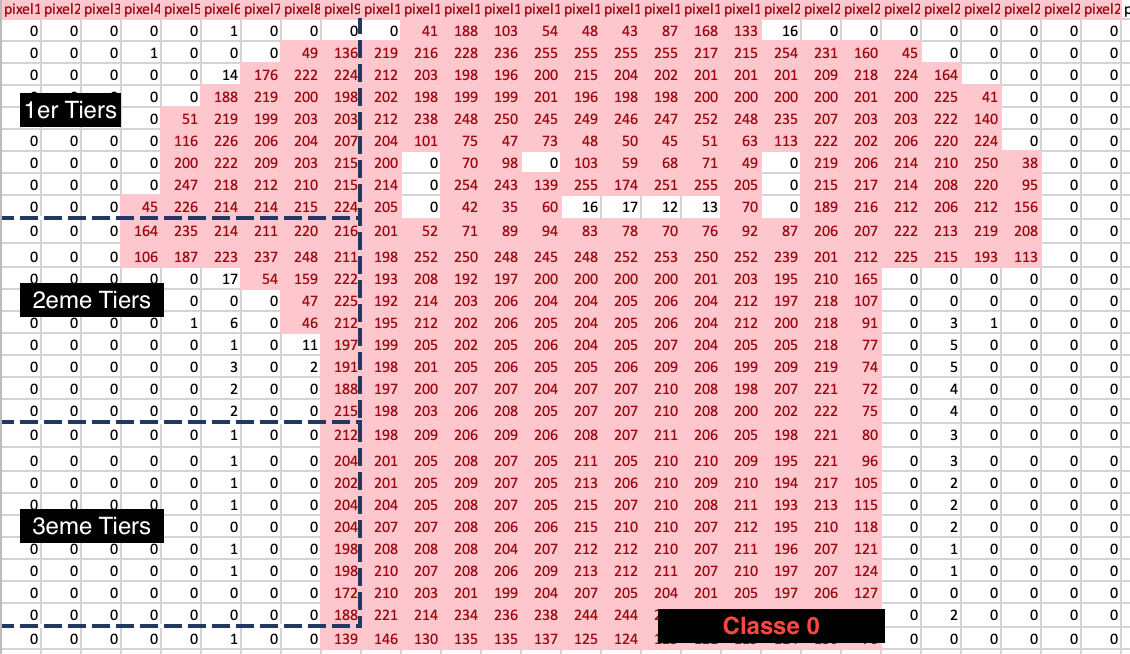
\includegraphics[scale = 0.15]{fichiers/decoupe_tshirt.png}		
		\end{minipage}\hfill

		\begin{minipage}{0.4\linewidth}
			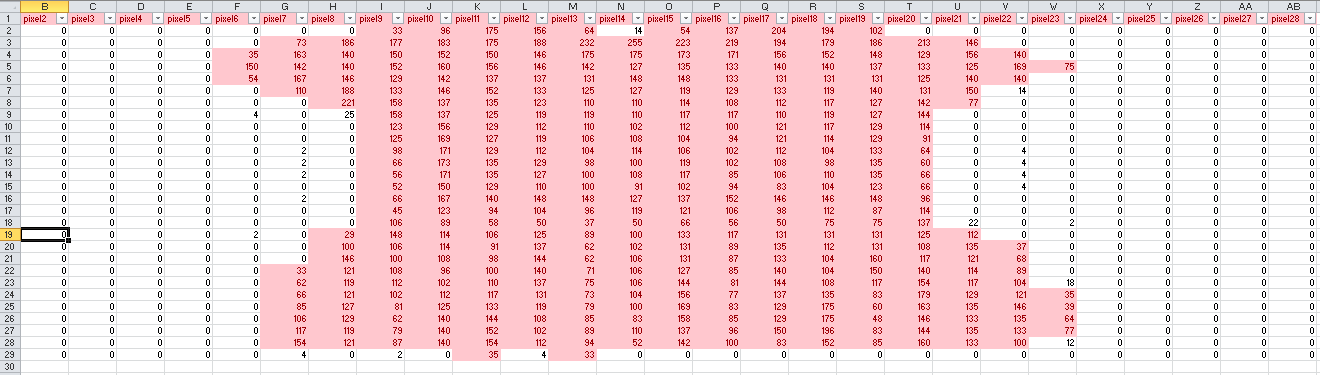
\includegraphics[scale = 0.15]{fichiers/ex_robe.PNG}		
		\end{minipage}\hfill
		\begin{minipage}{0.55\linewidth}
			Nous calculons aussi le nombre de pixels blancs formant un col. Car les tops ont des cols plus marqués que les robes.\\
		\end{minipage}

		\begin{minipage}{0.55\linewidth}
			Enfin, nous calculons le nombre de pixels non blancs pour les 2 tiers restants de l'image de l’image. Car nous avons remarqué que les robes sont moins "zoomées" que les t-shirts et un travail d'analyse a déjà été effecturé sur le 1er tiers (niveau col et manches), alors nous effectuons une analyse sur les 2 tiers restants de l'image.
		\end{minipage}\hfill
		\begin{minipage}{0.4\linewidth}
		%images
			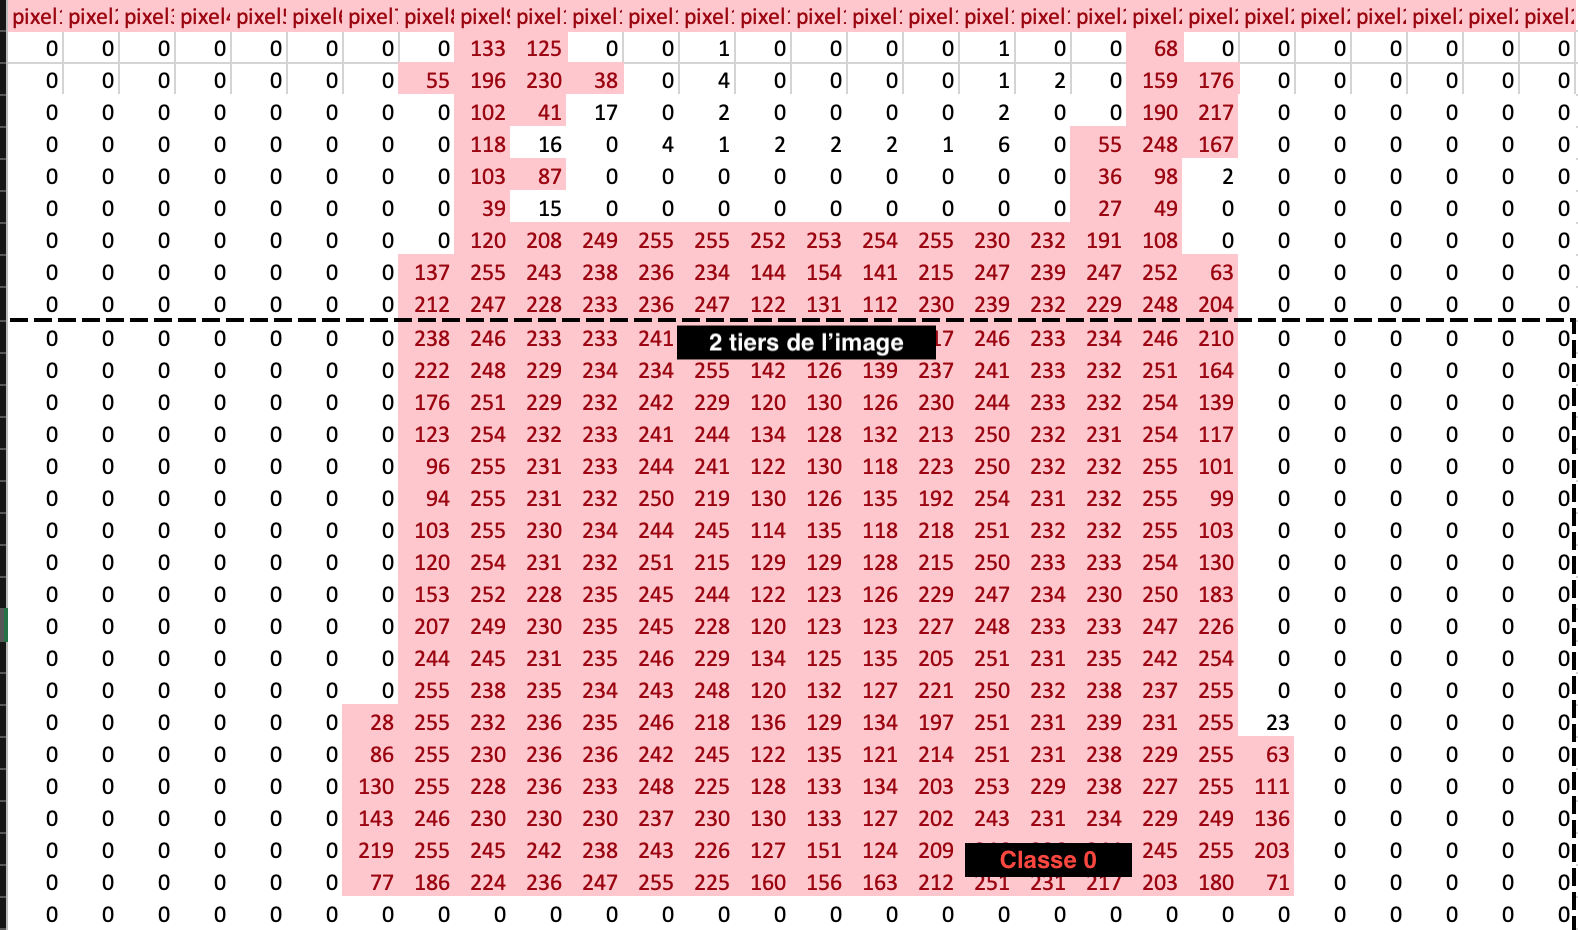
\includegraphics[scale = 0.10]{fichiers/ex_tshirt.png}	
		\end{minipage}
		
		Notre espace est donc le suivant :
		\begin{itemize}
			\item Pour l'axe $x$ : rapport des pixels non blancs sur les 1er tiers / pixels blancs du 3e tiers (gauche de l'image)
			\item Pour l'axe $y$ : nombre de pixels blancs niveau col
			\item Pour l'axe $z$ : nombre pixels colorés (2/3 image)
		\end{itemize}
		Nous évaluons pour l'axe $x$ le rapport de deux surfaces de 9x9 pixels tel que : \\
		Graphiquement :
		$$ \forall pixels_{i,j} < 25,  (\sum_{i=1} ^9 \sum_{j=1} ^9  (pixels_{i,j})) / (\sum_{i=19} ^{28} \sum_{j=1}^9  (pixels_{i,j}) ) $$
		Pour le jeu de données :
		$$ \forall pixels_j < 25, (\sum_{i=0} ^8 \sum_{j=1} ^9  (pixels_j +28i) ) / (\sum_{i=18} ^{27} \sum_{j=1} ^9  (pixels_j+28i) ) $$

	\subsection{Méthodes d'apprentissage utilisées}
		Chaque image sera caractérisée par les paramètres décrits dans la section ci- dessus. 
		\begin{itemize}
			\item Les K-NN (K plus proches voisins) : Fatima\\
			Un $k$ initial est fixé, la classification d'une nouvelle observation revient à calculer la distance de cette image avec ses $k$ plus proches voisins et l'étiquette de cette nouvelle observation sera déterminée selon l'étiquette la plus fréquente dans son voisinnage. Le $k$ optimal sera déterminé grâce à notre méthode d'optimisation décrite ci-après.\\
			\item La régression : Lauréline\\
			La variable $Y$ prend deux modalités possibles ${0, 1}$ selon la classe de l'objet qu'il décrit (0 pour $C_1$ et 1 pour $C_2$). On a la formule $Y = a + b_1 x_1+ b_2 x_2$ avec $x_1$ le rapport 1er tier / 3e tier et $x_2$ le rapport 2e tiers / 3e tiers. Notre algorithme déterminera et affinera les coefficients $b_1, b_2$ et la constante $a$ lors de l'apprentissage.
			\item SVM : Léa\\
			On cherche un hyperplan de dimension 2 (car nous travaillons dans espace de dimension 3), tel que pour tout objet $x$ de vecteur $x = {a_1, a_2} $ on a $h(x) = l_k (\sum_{i = 1} ^2 ((w_i . x_i ) + b ) )$ avec $w$ le vecteur de poids et $b$ le biais et $l_k$ le label tel que $l_k = 1 $ pour la classe $C_1$ et $l_k = -1$ pour la classe $C_2$. Grâce à cette équation d'hyperplan et en utilisant la norme Euclidienne de $w$, nous pouvons calculer la distance $d$ de l'hyperplan à chaque objet de l'espace. Et en déduire la marge (la distance minimale de $d$). Afin d'augmenter la tolérence aux variations de notre algorithme, nous cherchons l'hyperplan ayant la plus grande marge (l'hyperplan optimal). Ainsi, l'algorithme doit trouver le meilleur couple $(w, b)$ décrivant cet hyperplan. Pour facilité les calculs, nous allons normaliser l'équation de l'hyperplan.
		\end{itemize}
	\subsection{Méthode d'optimisation}
		Nous allons utiliser la méthode nested cross validation pour choisir les meilleurs paramètres de nos algorithmes.\\
		Nous allons utiliser la méthode de validation croisée pour assigner chaque donnée à une phase de d'apprentissage ou une phase de test. Cette méthode consiste à partitionner notre jeu de données en fonction d'une taille $k=5$. La répartition des parties ainsi créées à la phase d'apprentisage ou à la phase de test, l'entrainement de l'algorithme sur la phase d'apprentissage puis sur la phase de test pour laquelle nous comparerons les résultats obtenus aux résultats attendus. \\
		Nous définissons $k=5$ pour avoir un ratio acceptable entre le volume de données traitées et le temps d'éxecution.\\
		Nos parties seront stratifiées, c'est-à-dire qu'elles contiennent la même proportion de chaque classe étudiées, afin d'avoir une chance équiprobable d'évaluer un objet issu de la classe $C_1$ ou de la classe $C_2$.\\
		Avec la méthode KNN, nous allons comparer la performance pour le jeu de données en utilisant les 3 dimensions décrites dans le rapport et les 784 dimensions correspondant aux pixels de l'image. 
	\subsection{Protocole de comparaison}
		Pour comparer les résultats des différentes méthodes d'apprentissages utilisées, nous évaluons leur taux d’erreurs respectifs sur des jeux identiques de données ainsi que leur temps de traitement.


\end{document}